\documentclass[tikz,border=3pt]{standalone}
\usepackage{pgfplots}
\usepgfplotslibrary{groupplots}
\pgfplotsset{compat=1.18}
\begin{document}
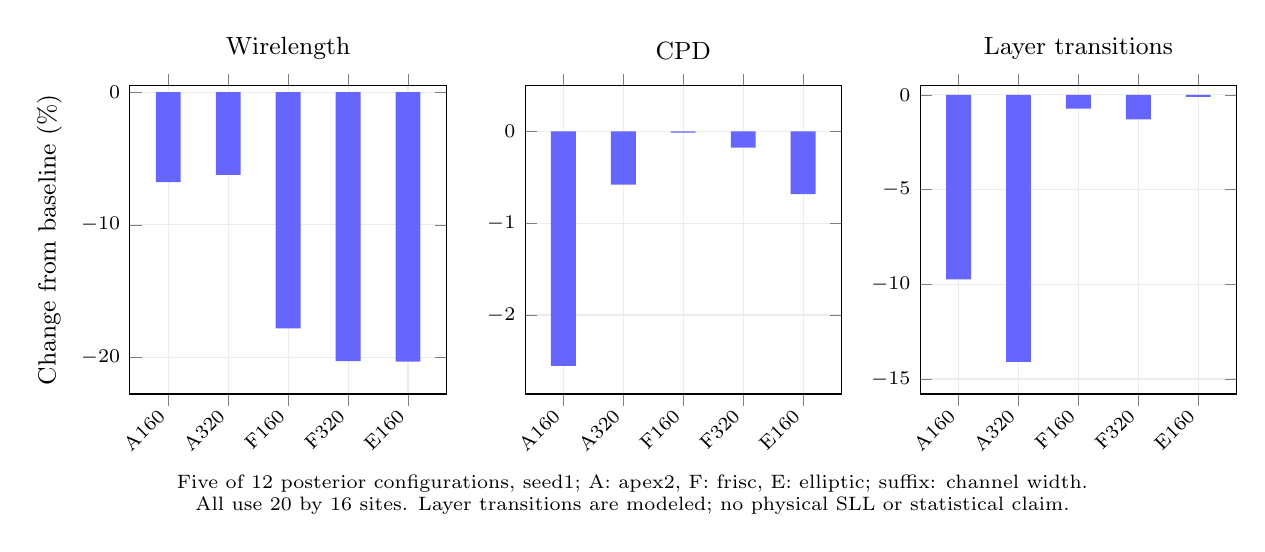
\begin{tikzpicture}
\begin{groupplot}[group style={group size=3 by 1,horizontal sep=1cm},width=5.6cm,height=5.5cm,ybar,/pgf/bar width=9pt,xtick={1,2,3,4,5},xticklabels={A160,A320,F160,F320,E160},xticklabel style={rotate=45,anchor=east},enlarge x limits=.16,grid=major,grid style={gray!15},tick label style={font=\scriptsize},label style={font=\small},title style={font=\small}]
\nextgroupplot[title={Wirelength},ylabel={Change from baseline (\%)},ymin=-22.73826829440406,ymax=.5]
\addplot[fill=blue!60,draw=none] coordinates {(1,-6.789020626928699) (2,-6.245568101238208) (3,-17.808311443389236) (4,-20.263648284905788) (5,-20.302025262860766)};
\nextgroupplot[title={CPD},ymin=-2.859033752481802,ymax=.5]
\addplot[fill=blue!60,draw=none] coordinates {(1,-2.552708707573037) (2,-0.5798741248850825) (3,-0.012826679493349591) (4,-0.17650267963159605) (5,-0.6843879284591292)};
\nextgroupplot[title={Layer transitions},ymin=-15.789310611928734,ymax=.5]
\addplot[fill=blue!60,draw=none] coordinates {(1,-9.733777038269553) (2,-14.097598760650653) (3,-0.7311586051743535) (4,-1.2965050732807182) (5,-0.10632642211589882)};
\end{groupplot}
\node[anchor=north,font=\scriptsize,align=center] at (current bounding box.south) {Five of 12 posterior configurations, seed1; A: apex2, F: frisc, E: elliptic; suffix: channel width.\\All use 20 by 16 sites. Layer transitions are modeled; no physical SLL or statistical claim.};
\end{tikzpicture}
\end{document}
